\chapter{Neural networks}
The topics presented in this thesis are based on neural networks, especially convolutional neural networks, which are a distinct neural network variation for image processing using filters.
Here we provide a very brief high-level overview of some of the concepts that are important for the later chapters, but a more detailed overview of deep learning and neural networks can be found, for example, in \citep{deep-learning}.

\section{Convolutional Neural Networks}
The most significant component of Convolutional Neural Networks (CNNs) is the convolutional layers that are their primary building block.
Using convolutional filters allows neural networks to extract useful information from images to accomplish various tasks.
The convolutional blocks are based on the mathematical convolution operation of capturing the signal of pre-determined window size.
A CNN classifier often consists of multiple convolutional layers with other layers in between.
Successive convolutional layers build on top of one another, and the deeper layers get high activations on more specific features.
In many final models, the earlier layers are thus somewhat similar and re-usable as they often detect relatively primitive shapes, like diagonal or horizontal lines.
In this thesis, we often talk about the parameters or the weights of a network.
The number of parameters in a network tells how complex it is and how expensive it is to store.
The floating-point numbers in the various layers are these weights, which are generally 32-bit numbers, but their precision can vary.

\subsection{Parameters}
To get the total number of parameters required for a single convolutional layer, we need to determine the input size, convolution window size, and the number of filters.
For example, if the input is a 256x256 RGB image, the input size is 256x256x3.
Now, if we apply 16 filters with a window size of 5, each of the filters requires 5x5x3 parameters, bringing the total to 1200 parameters.
A fully connected layer with 1000 hidden units would require a matrix with around 200 million parameters, so it would not really be possible even to apply multiple of these layers while maintaining the image size.
The convolution allows for keeping the dimensions between successive layers and only modifying the number of channels between the layers.
Often convolutional models reduce the first two dimensions, and the number of channels increases in the deeper layers.
For this, the convolutions can use a stride parameter to skip some positions for the convolution.
The pooling layer is another way to reduce the size.
Generally used pooling layers are average and maximum pool layers. 
They are applied similarly to a convolution but capture the average or the maximum of a window.
Neither of these approaches requires any extra learnable weights.


\subsection{Embedding}
Generally, the role of the convolutional layers in a CNN model is to act as a feature extractor.
As can be seen in the number of parameters of the fully connected layer on a full-sized image, the image needs to have a smaller dense representation in order to connect a linear layer to it.
This representation can be generated with the convolutional layers.
The final representation that can be pushed into a linear classifier for some final inference is called an image embedding.
Embeddings are representations of things in relatively small continuous numbered vectors, here we consider embeddings of images, but embeddings are used, for example, for words and sentences as well.
Besides just doing classification, the embeddings can represent things, for example, faces or objects.
When a general embedding is generated it can be used to for example to evaluate if someone is the same person as the embedding or to find similar images.

\begin{figure}[h!] 
\centering 
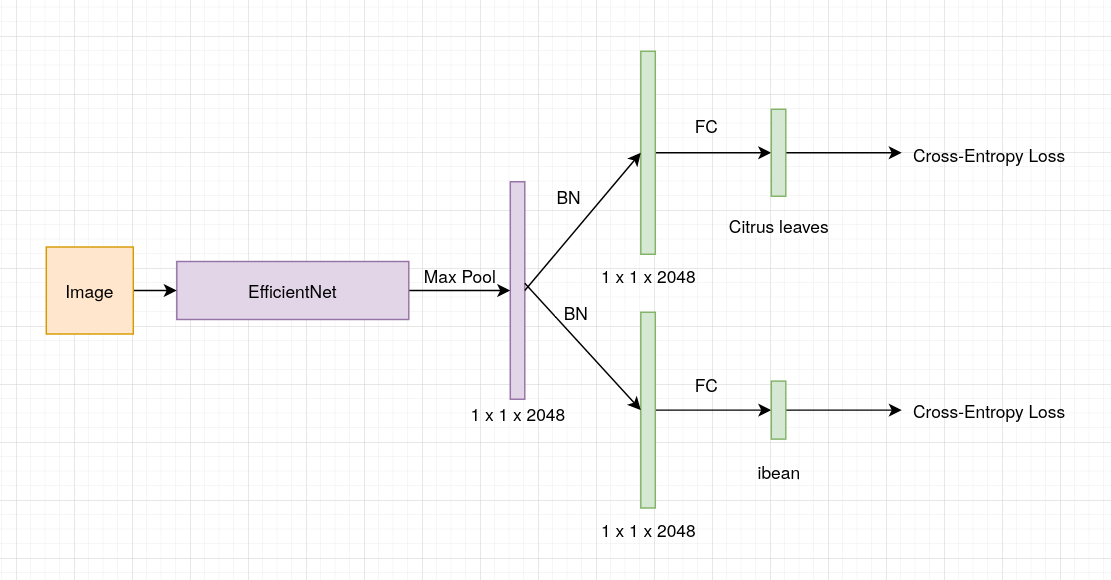
\includegraphics[width=0.8\textwidth]{imgs/object_classification_architecture.png}
\caption{Image of an example of a convolutional neural network architecture with backbone (a), image classifier (b) and task head (c) labeled. TODO: IMAGE}
\end{figure}

\subsection{Backbone}
The feature extraction part of a convolutional classifier is called the backbone.
Finding better features is often correlated with more parameters and a larger model, but various architectural decisions can also help.
The largest convolutional models have thousands of layers.
Best models often use as large backbones as is possible within the constraints of the specific deployment.
The backbone is thus responsible for creating the image embedding that is used to produce an output.
Some tasks require feature maps taken from the middle of the backbone instead of only relying on the final layer.

\subsection{Head}
The final layers of a classifier are called the head.
The head is responsible for producing the output, and its exact architecture varies from task to task.
It could be just a single linear layer connecting the image embedding to final class probability distribution or an image segmentation model classifying each pixel in the image.
The head can thus contain whatever layers are needed to get the output, combining batch normalization, dropout, convolutional, recurrent, and linear layers depending on what is needed to solve the task.
An example visualization of how the different parts of a convolutional model are connected is shown in Figure 2.1.
The architecture would vary on a task-by-task basis, and the figure shows a basic image classifier architecture.


